\documentclass[12pt,a4paper]{article}

% Encoding and fonts
\usepackage[utf8]{inputenc}
\usepackage[T1]{fontenc}
\usepackage{lmodern}

% Mathematics
\usepackage{amsmath}
\usepackage{amssymb}
\usepackage{amsfonts}
\usepackage{amsthm}
\usepackage{mathtools}

% Layout
\usepackage[margin=1in]{geometry}
\usepackage{setspace}
\doublespacing
\emergencystretch=2em

% References and links
\usepackage[hidelinks]{hyperref}

% Figures
\usepackage{graphicx}
\graphicspath{{figures/}}
\usepackage{float}
\usepackage[hypcap=true]{caption}

% Theorem environments
\newtheorem{theorem}{Theorem}[section]
\newtheorem{proposition}[theorem]{Proposition}
\newtheorem{lemma}[theorem]{Lemma}
\newtheorem{corollary}[theorem]{Corollary}
\theoremstyle{definition}
\newtheorem{definition}[theorem]{Definition}
\theoremstyle{remark}
\newtheorem{remark}[theorem]{Remark}
\newtheorem{conjecture}[theorem]{Conjecture}

% Title information
\title{Information Geometry of the Quantum-Classical Transition in Photosynthetic Exciton Transport}
\author{Ian Todd\\
Sydney Medical School\\
University of Sydney\\
Sydney, NSW, Australia\\
\texttt{itod2305@uni.sydney.edu.au}}
\date{}

\begin{document}

\maketitle

\begin{abstract}
Decoherence drives the quantum-to-classical transition, but its information-geometric structure---the precise dimensional and metric changes it imposes on quantum state space---has not been quantified in the Bures/Fisher--Rao framework. We show that decoherence is a dimensional collapse: the dephasing channel maps a $(d^2{-}1)$-dimensional quantum manifold onto the $(d{-}1)$-dimensional classical probability simplex, annihilating the $d^2{-}d$ coherence directions while preserving the $d{-}1$ population dimensions. At diagonal states, the classical and quantum tangent subspaces are Bures-orthogonal. We compute the exact Bures principal angle $\theta_B$ between these subspaces at every full-rank qubit state, obtaining $\cos^2\theta_B = r_z^2 r_\perp^2/[(1{-}r_\perp^2)(1{-}r_z^2)]$, where $r_z$ is the population imbalance and $r_\perp$ the coherence magnitude. For $d \geq 3$, we prove that Bures-orthogonality holds if and only if $\rho$ is diagonal---any coherence breaks the clean classical-quantum split. We apply this framework to the Fenna--Matthews--Olson photosynthetic complex ($d = 7$), where decoherence collapses 48 quantum dimensions to 6 classical dimensions. Using a Haken--Strobl model with reaction-centre trapping, we compute transport efficiency and the six Bures principal angles from the same sink-inclusive dynamics, with the geometry extracted from the renormalized conditional state. At the ENAQT-optimal dephasing rate ($\gamma_{\mathrm{opt}} \approx 100$--$150$\,cm$^{-1}$), all principal angles exceed $87^\circ$: biologically optimal transport occurs in a regime that is geometrically close to classical, with strong quantum-classical mixing confined to weaker dephasing ($\gamma \lesssim 10$\,cm$^{-1}$).
\end{abstract}

%% ============================================================
\section{Introduction}
\label{sec:intro}

The quantum-to-classical transition mediated by decoherence \cite{zeh1970interpretation,zurek1981pointer,zurek2003decoherence,schlosshauer2005decoherence} is not merely a theoretical curiosity in biological systems---it is functionally relevant. Photosynthetic complexes exploit quantum coherence during energy transfer on femtosecond timescales \cite{engel2007evidence}, and optimal transport efficiency occurs at intermediate dephasing rates, a phenomenon termed environment-assisted quantum transport (ENAQT) \cite{plenio2008dephasing,rebentrost2009environment,mohseni2008environment}. The quantum biology literature has established that partial decoherence can enhance biological function \cite{cao2020quantum}, but the geometric structure of this transition---how many degrees of freedom are destroyed, how cleanly classical information separates from quantum information, and what the dimensional architecture of intermediate regimes looks like---has not been quantified.

Information geometry provides the natural mathematical language for these questions. The quantum Fisher information matrix (QFIM) \cite{liu2020quantum,braunstein1994statistical} measures the dimensionality of distinguishable quantum states, and the Bures metric it induces \cite{bures1969extension,uhlmann1976transition,petz1996monotone} is the unique minimal monotone Riemannian metric on quantum state space. The classical Fisher--Rao metric \cite{rao1945information,chentsov1982statistical,amari1985differential} plays the analogous role for probability distributions. Despite the maturity of both decoherence theory and information geometry, these frameworks have not been combined to characterize the dimensional structure of the quantum-to-classical transition.

In this paper, we show that decoherence is a \emph{dimensional collapse} in the information-geometric sense. A $d$-dimensional quantum system lives on a $(d^2{-}1)$-dimensional state manifold equipped with the Bures metric. Decoherence projects this manifold onto the $(d{-}1)$-dimensional classical probability simplex equipped with the Fisher--Rao metric. Specifically:
\begin{enumerate}
\item[\emph{(Collapse.)}] The decoherence channel reduces the QFIM rank from $d^2{-}1$ to at most $d{-}1$ (Theorem~\ref{thm:dim-collapse}), and the Bures metric restricts to the Fisher--Rao metric on $\Delta_{d-1}$ (Theorem~\ref{thm:metric-restriction}). At full-rank diagonal states, the differential of the dephasing map is the Bures-orthogonal projector onto the classical tangent subspace (Theorem~\ref{thm:orthogonal-decomposition}).
\item[\emph{(Geometry of the split.)}] We compute the exact Bures principal angle $\theta_B$ between the classical and quantum tangent subspaces at every full-rank qubit state (Theorem~\ref{thm:bures-angle}). For $d \geq 3$, we prove that Bures-orthogonality holds if and only if $\rho$ is diagonal (Theorem~\ref{thm:global-orthogonality}), and a perturbative formula quantifies the departure (Theorem~\ref{thm:qudit-angles}).
\item[\emph{(Application.)}] We apply the framework to the Fenna--Matthews--Olson (FMO) photosynthetic complex, where $d = 7$ sites yield a collapse from 48 to 6 information-geometric dimensions. Computing transport efficiency and the six Bures principal angles from the same sink-inclusive dynamics, we find that at the ENAQT-optimal dephasing rate the system is geometrically nearly classical (all angles $> 87^\circ$), with the strong quantum-classical mixing regime lying at much weaker dephasing.
\end{enumerate}

The paper is organized as follows. Section~\ref{sec:geometry} establishes the information-geometric framework. Section~\ref{sec:decoherence} contains the core mathematical results. Section~\ref{sec:thermodynamics} derives the thermodynamic cost of dimensional collapse. Section~\ref{sec:fmo} applies the framework to the FMO complex. Section~\ref{sec:discussion} discusses implications, limitations, and connections to classical biological coherence.

%% ============================================================
\section{Information-Geometric Framework}
\label{sec:geometry}

We establish the mathematical framework that makes ``dimensional collapse'' precise.

\begin{definition}[Quantum state manifold]
\label{def:state-manifold}
The space of $d \times d$ density matrices,
\begin{equation}
\label{eq:state-manifold}
\mathcal{M}_Q = \bigl\{\rho \in \mathbb{C}^{d \times d} : \rho \geq 0,\; \mathrm{Tr}\,\rho = 1\bigr\},
\end{equation}
is a real manifold of dimension $d^2 - 1$: a $d \times d$ Hermitian matrix has $d^2$ real parameters, the trace constraint removes one, leaving $d - 1$ populations and $d(d{-}1)$ coherences.
\end{definition}

\begin{definition}[Quantum Fisher information matrix]
\label{def:qfim}
Let $\rho(\theta)$ be a smooth parametric family of density matrices with $\theta \in \mathbb{R}^p$. The QFIM is the $p \times p$ matrix with entries
\begin{equation}
\label{eq:qfim}
[F_Q]_{ij} = \mathrm{Tr}\!\left[\rho\,\frac{L_i L_j + L_j L_i}{2}\right],
\end{equation}
where $L_i$ is the symmetric logarithmic derivative (SLD) defined by $\partial_i \rho = (\rho L_i + L_i \rho)/2$. For full-rank $\rho$ with eigenbasis $\rho = \sum_k p_k |k\rangle\langle k|$, the matrix elements are $(L_i)_{mn} = 2(\partial_i \rho)_{mn}/(p_m + p_n)$.
\end{definition}

The QFIM defines the Bures--Helstrom metric $ds^2_{\mathrm{Bures}} = \frac{1}{4}\sum_{ij} [F_Q]_{ij}\, d\theta^i\, d\theta^j$, the unique minimal monotone Riemannian metric on quantum state space \cite{petz1996monotone,braunstein1994statistical}. By Petz's monotonicity theorem, for any CPTP map $\Lambda$:
\begin{equation}
\label{eq:dpi}
F_Q\bigl(\Lambda[\rho(\theta)]\bigr) \leq F_Q\bigl(\rho(\theta)\bigr)
\end{equation}
in the L\"owner order---quantum channels cannot increase statistical distinguishability.

\begin{definition}[Effective quantum dimensionality]
\label{def:deff}
Given a QFIM $F_Q$ with eigenvalues $\lambda_1 \geq \cdots \geq \lambda_p \geq 0$, the effective quantum dimensionality is the participation ratio
\begin{equation}
\label{eq:deff}
D_{\mathrm{eff}}^Q = \frac{\bigl(\sum_i \lambda_i\bigr)^2}{\sum_i \lambda_i^2},
\end{equation}
ranging from $1$ (single dominant direction) to $p$ (all directions equally estimable). $D_{\mathrm{eff}}^Q$ is a coordinate-dependent diagnostic: the rank of $F_Q$ is invariant, but the participation ratio depends on the parameterization. The main theorems of this paper depend only on rank, kernel structure, and metric properties.
\end{definition}

%% ============================================================
\section{Decoherence as Dimensional Projection}
\label{sec:decoherence}

We now show that decoherence acts as a geometric projection, annihilating the $d^2 - d$ off-diagonal directions and collapsing quantum state space onto the $(d{-}1)$-dimensional classical probability simplex.

\begin{definition}[Decoherence channel]
\label{def:decoherence-channel}
Fix an orthonormal pointer basis $\{|k\rangle\}_{k=1}^d$. The complete dephasing channel is
\begin{equation}
\label{eq:dephasing}
\Lambda_{\mathrm{dec}}(\rho) = \sum_{k=1}^d |k\rangle\langle k|\, \rho\, |k\rangle\langle k|,
\end{equation}
setting all off-diagonal elements to zero: $[\Lambda_{\mathrm{dec}}(\rho)]_{kl} = \delta_{kl}\, \langle k|\rho|k\rangle$.
\end{definition}

\begin{theorem}[Dimensional collapse]
\label{thm:dim-collapse}
Let $\mathcal{M}_Q$ be the quantum state manifold of a $d$-dimensional system $(\dim \mathcal{M}_Q = d^2 - 1)$. The decoherence channel $\Lambda_{\mathrm{dec}}$ maps $\mathcal{M}_Q$ onto the classical probability simplex $\Delta_{d-1}$ $(\dim \Delta_{d-1} = d-1)$. Specifically:

\begin{enumerate}
\item[\emph{(i)}] The image $\Lambda_{\mathrm{dec}}(\mathcal{M}_Q) = \Delta_{d-1}$.

\item[\emph{(ii)}] The $d^2 - d$ off-diagonal parameters become unestimable: for any smooth parameterization $\theta = (\theta_{\mathrm{diag}}, \theta_{\mathrm{off}})$, the QFIM of $\Lambda_{\mathrm{dec}}[\rho(\theta)]$ satisfies
\begin{equation}
\label{eq:offdiag-vanish}
[F_Q(\Lambda_{\mathrm{dec}}[\rho])]_{\alpha\beta} = 0 \quad \text{whenever } \alpha \in \theta_{\mathrm{off}} \text{ or } \beta \in \theta_{\mathrm{off}}.
\end{equation}
In particular, $\mathrm{rank}\, F_Q(\Lambda_{\mathrm{dec}}[\rho]) \leq d - 1$.

\item[\emph{(iii)}] The dimensional collapse ratio is
\begin{equation}
\label{eq:collapse-ratio}
\frac{\dim \Delta_{d-1}}{\dim \mathcal{M}_Q} = \frac{d-1}{d^2-1} = \frac{1}{d+1},
\end{equation}
which vanishes as $d \to \infty$.
\end{enumerate}
\end{theorem}

\begin{proof}
Part~(i): $\Lambda_{\mathrm{dec}}$ sends $\rho$ to $\mathrm{diag}(\langle k|\rho|k\rangle)$, a point in $\Delta_{d-1}$; every point in $\Delta_{d-1}$ is the image of some diagonal state. Part~(iii) is arithmetic.

For Part~(ii): the decohered state depends only on $\theta_{\mathrm{diag}}$, so $\partial \rho_{\mathrm{dec}}/\partial \theta_{\mathrm{off}}^\alpha = 0$, giving $L_\alpha = 0$ and hence $[F_Q]_{\alpha\beta} = 0$ whenever $\alpha$ or $\beta$ is off-diagonal. The surviving diagonal block reduces to the classical Fisher information:
\begin{equation}
\label{eq:qfim-classical}
[F_Q]_{ij}^{\mathrm{diag}} = \sum_{k=1}^d \frac{1}{p_k}\, \frac{\partial p_k}{\partial \theta_{\mathrm{diag}}^i}\, \frac{\partial p_k}{\partial \theta_{\mathrm{diag}}^j} = [F_{\mathrm{cl}}]_{ij},
\end{equation}
which has rank at most $d - 1$.
\end{proof}

\begin{theorem}[Metric restriction]
\label{thm:metric-restriction}
Under $\Lambda_{\mathrm{dec}}$, the Bures metric on $\mathcal{M}_Q$ restricts to the Fisher--Rao metric on $\Delta_{d-1}$:
\begin{equation}
\label{eq:metric-restriction}
ds^2_{\mathrm{Bures}}\big|_{\Delta_{d-1}} = \frac{1}{4} \sum_{k=1}^d \frac{dp_k^2}{p_k} = \frac{1}{4}\, ds^2_{\mathrm{Fisher\text{-}Rao}}.
\end{equation}
\end{theorem}

\begin{proof}
For diagonal states, the SLD is diagonal: $\langle k|L_i|k\rangle = (\partial_i p_k)/p_k$. The Bures line element becomes $\frac{1}{4}\sum_k dp_k^2/p_k$, the Fisher--Rao metric \cite{braunstein1994statistical}.
\end{proof}

\begin{theorem}[Orthogonal decomposition]
\label{thm:orthogonal-decomposition}
Let $\rho = \mathrm{diag}(p_1, \ldots, p_d)$ be a full-rank diagonal state. The tangent space admits an orthogonal decomposition under the Bures metric:
\begin{equation}
\label{eq:orthogonal-decomposition}
T_\rho \mathcal{M}_Q = T_\rho^{\mathrm{diag}} \oplus T_\rho^{\mathrm{off}},
\end{equation}
where $T_\rho^{\mathrm{diag}}$ is the $(d{-}1)$-dimensional traceless diagonal subspace and $T_\rho^{\mathrm{off}}$ is the $(d^2{-}d)$-dimensional off-diagonal Hermitian subspace. The differential $d\Lambda_{\mathrm{dec}}|_\rho$ acts as the identity on $T_\rho^{\mathrm{diag}}$ and as zero on $T_\rho^{\mathrm{off}}$, so it is the $g_B$-orthogonal projector onto $T_\rho^{\mathrm{diag}}$.
\end{theorem}

\begin{proof}
At a diagonal state, any traceless Hermitian $X$ decomposes as $X = X_D + X_O$ (diagonal + off-diagonal). The SLD for a diagonal perturbation $X_D$ is diagonal: $(L_{X_D})_{kk} = x_k/p_k$. The SLD for an off-diagonal perturbation $X_O$ is off-diagonal: $(L_{X_O})_{mn} = 2z_{mn}/(p_m + p_n)$ for $m \neq n$. The anticommutator $\{L_{X_D}, L_{X_O}\}$ is off-diagonal (product of diagonal and off-diagonal matrices), so $\rho \{L_{X_D}, L_{X_O}\}$ is off-diagonal with zero trace:
\[
g_B(X_D, X_O) = \frac{1}{4}\,\mathrm{Tr}\!\left[\rho\,\frac{\{L_{X_D}, L_{X_O}\}}{2}\right] = 0.
\]
The dephasing channel preserves diagonal and annihilates off-diagonal perturbations, completing the identification as orthogonal projector.
\end{proof}

\subsection{The classical--quantum split away from the simplex}
\label{sec:bures-angle}

Theorem~\ref{thm:orthogonal-decomposition} establishes orthogonality at diagonal states. What happens at states carrying coherence? For qubits, a single principal angle characterizes the full relationship.

\begin{theorem}[Bures separation angle]
\label{thm:bures-angle}
Let $\rho = (I + \mathbf{r} \cdot \boldsymbol{\sigma})/2$ be a full-rank qubit state $(|\mathbf{r}| < 1)$ with coherence magnitude $r_\perp = \sqrt{r_x^2 + r_y^2}$ and population imbalance $r_z$. The principal angle $\theta_B$ between $T_\rho^{\mathrm{diag}}$ and $T_\rho^{\mathrm{off}}$ under the Bures metric satisfies
\begin{equation}
\label{eq:bures-angle}
\cos^2 \theta_B = \frac{r_z^2\, r_\perp^2}{(1 - r_\perp^2)(1 - r_z^2)}.
\end{equation}
Equivalently,
\begin{equation}
\label{eq:bures-angle-sin}
\sin^2 \theta_B = \frac{1 - |\mathbf{r}|^2}{(1 - r_\perp^2)(1 - r_z^2)}.
\end{equation}
\end{theorem}

\begin{proof}
The Bures metric on qubit state space in Bloch coordinates is $g_{ij}^B = \frac{1}{4}[\delta_{ij} + r_i r_j/(1 - |\mathbf{r}|^2)]$. The principal angle is found by maximizing $g_B(\hat{e}_z, v)/(\|\hat{e}_z\| \cdot \|v\|)$ over $v \in T_\rho^{\mathrm{off}}$. The maximizer is $v_\perp = (r_x, r_y, 0)/r_\perp$. Computing:
\begin{align*}
g_B(\hat{e}_z, v_\perp) &= \frac{r_z r_\perp}{4(1 - |\mathbf{r}|^2)}, \\
g_B(\hat{e}_z, \hat{e}_z) &= \frac{1 - r_\perp^2}{4(1 - |\mathbf{r}|^2)}, \\
g_B(v_\perp, v_\perp) &= \frac{1 - r_z^2}{4(1 - |\mathbf{r}|^2)}.
\end{align*}
The squared cosine follows; the sine formula uses $(1 - r_\perp^2)(1 - r_z^2) - r_z^2 r_\perp^2 = 1 - |\mathbf{r}|^2$.
\end{proof}

\begin{corollary}[Structure of the classical--quantum split]
\label{cor:angle-structure}
\quad
\begin{enumerate}
\item[\emph{(i)}] $\theta_B = \pi/2$ if and only if $r_\perp = 0$ or $r_z = 0$: subspaces are Bures-orthogonal at all diagonal and all equatorial states.
\item[\emph{(ii)}] $\theta_B < \pi/2$ if and only if both $r_\perp \neq 0$ and $r_z \neq 0$.
\item[\emph{(iii)}] Dephasing monotonically increases $\theta_B$ toward $\pi/2$.
\end{enumerate}
\end{corollary}

\begin{proof}
Parts (i)--(ii) are immediate from~\eqref{eq:bures-angle}. For~(iii): under dephasing, $r_\perp \mapsto (1{-}2\gamma)r_\perp$ while $r_z$ is preserved. The numerator of $\cos^2\theta_B$ decreases monotonically and the denominator increases, so $\theta_B$ increases.
\end{proof}

\begin{corollary}[Estimation-theoretic interpretation]
\label{cor:estimation}
For a full-rank qubit state, the quantum Fisher information for the population parameter $r_z$ is $[F_Q]_{zz} = (1 - r_\perp^2)/(1 - |\mathbf{r}|^2)$. When the coherence parameters are eliminated via the Schur complement \cite{zhang2025hybrid,albarelli2019restoring}, the effective Fisher information is
\begin{equation}
\label{eq:fzz-eff}
[F_Q]_{zz}^{\mathrm{eff}} = [F_Q]_{zz}\,\sin^2\theta_B = \frac{1}{1 - r_z^2}.
\end{equation}
The Bures separation angle determines the fraction of SLD Fisher information for the population parameter that survives elimination of coherence nuisance parameters.
\end{corollary}

\begin{proof}
The full QFIM is $F_Q = I + \mathbf{r}\mathbf{r}^T/(1 - |\mathbf{r}|^2)$. By Sherman--Morrison, $(F_Q^{-1})_{zz} = 1 - r_z^2$. The Schur complement gives $[F_Q]_{zz}^{\mathrm{eff}} = 1/(1 - r_z^2)$. The ratio $[F_Q]_{zz}^{\mathrm{eff}}/[F_Q]_{zz} = (1 - |\mathbf{r}|^2)/[(1 - r_\perp^2)(1 - r_z^2)] = \sin^2\theta_B$.
\end{proof}

\subsection{Generalization to qudits}
\label{sec:qudit-angles}

For $d$-dimensional systems, there are $d - 1$ principal angles between $T_\rho^{\mathrm{diag}}$ and $T_\rho^{\mathrm{off}}$. Theorem~\ref{thm:orthogonal-decomposition} shows these are all $\pi/2$ at diagonal states. For $d \geq 3$, the converse holds exactly:

\begin{theorem}[Global orthogonality criterion for $d \geq 3$]
\label{thm:global-orthogonality}
For $d \geq 3$, a full-rank state $\rho$ achieves the Bures-orthogonal decomposition $T_\rho^{\mathrm{diag}} \perp_{g_B} T_\rho^{\mathrm{off}}$ if and only if $\rho$ is diagonal in the pointer basis.
\end{theorem}

\begin{proof}
The reverse direction is Theorem~\ref{thm:orthogonal-decomposition}. For the forward direction, assume orthogonality holds. Define the Jordan product map $\mathcal{J}_\rho(L) = (\rho L + L\rho)/2$, which is invertible on Hermitian matrices when $\rho$ is full-rank. The SLD for tangent vector $X$ is $L_X = \mathcal{J}_\rho^{-1}(X)$.

For any traceless diagonal $X_D = \mathrm{diag}(x_1, \ldots, x_d)$ and off-diagonal Hermitian $X_O$, the SLD metric identity gives
\begin{equation}
\label{eq:sld-identity}
g_B(X_D, X_O) = \tfrac{1}{2}\sum_k x_k\, (L_{X_O})_{kk}.
\end{equation}
Since this vanishes for all traceless $x$, orthogonality requires $(L_{X_O})_{kk}$ to be constant across $k$---the diagonal of $L_{X_O}$ is flat. Hence $L_{X_O} = c I + Z$ for some $c \in \mathbb{R}$ and $Z$ off-diagonal.

Let $\mathcal{O}$ denote the $d(d{-}1)$-dimensional space of off-diagonal Hermitian matrices and $\mathcal{W} = \mathbb{R}I \oplus \mathcal{O}$. The flat-diagonal condition means $S := \mathcal{J}_\rho^{-1}(\mathcal{O}) \subset \mathcal{W}$. Consider the projection $\pi\colon \mathcal{W} \to \mathcal{O}$ defined by $cI + Z \mapsto Z$. This is injective on $S$: if $cI \in S$ then $\mathcal{J}_\rho(cI) = c\rho \in \mathcal{O}$, but $\rho$ has positive diagonal entries, forcing $c = 0$. Since $\dim S = \dim \mathcal{O} = d(d{-}1)$, the restricted projection $\pi|_S$ is an isomorphism.

Therefore, for every $Z \in \mathcal{O}$ there exists a unique $c(Z) \in \mathbb{R}$ with $c(Z)I + Z \in S$, meaning $\mathcal{J}_\rho(c(Z)I + Z) \in \mathcal{O}$. Taking the diagonal:
\begin{equation}
\label{eq:diag-constraint}
\mathrm{diag}(\rho Z + Z\rho) = -2c(Z)\, p, \qquad p = (p_1, \ldots, p_d) = \mathrm{diag}(\rho).
\end{equation}
Now substitute the basis elements. For $R_{kl} = |k\rangle\langle l| + |l\rangle\langle k|$:
\begin{equation}
\label{eq:diag-Rkl}
\mathrm{diag}(\rho R_{kl} + R_{kl}\rho) = 2\,\mathrm{Re}(\rho_{kl})\,(e_k + e_l),
\end{equation}
and for $I_{kl} = i|k\rangle\langle l| - i|l\rangle\langle k|$:
\begin{equation}
\label{eq:diag-Ikl}
\mathrm{diag}(\rho I_{kl} + I_{kl}\rho) = 2\,\mathrm{Im}(\rho_{kl})\,(e_k + e_l).
\end{equation}
If $\rho_{kl} \neq 0$, at least one of these is nonzero, so $e_k + e_l \in \mathrm{span}\{p\}$. But for $d \geq 3$, the vector $e_k + e_l$ has $d - 2 \geq 1$ zero entries while $p$ has all entries strictly positive, so $e_k + e_l$ cannot be proportional to $p$. Contradiction; hence $\rho_{kl} = 0$ for all $k \neq l$.
\end{proof}

\begin{remark}[The qubit exception]
\label{rem:qubit-exception}
For $d = 2$, the vector $e_1 + e_2 = (1,1)$ is proportional to $p = (p_1, p_2)$ if and only if $p_1 = p_2$, recovering the qubit result: equatorial states ($r_z = 0$) achieve Bures-orthogonality despite carrying coherence (Corollary~\ref{cor:angle-structure}(i)). The proof above shows that $d \geq 3$ eliminates this loophole.
\end{remark}

Theorem~\ref{thm:global-orthogonality} settles the qualitative question: for $d \geq 3$, any coherence breaks orthogonality. We now quantify \emph{how much} the subspaces mix.

\begin{theorem}[Perturbative cross-Gram near the simplex]
\label{thm:qudit-angles}
Let $\rho = \mathrm{diag}(p) + C$ be a full-rank $d$-dimensional state with off-diagonal part $C$.
\begin{enumerate}
\item[\emph{(i)}] Near the simplex ($\|C\|$ small), the cross-Gram matrix has entries
\begin{equation}
\label{eq:cross-gram}
g_B(D_a, R_{kl}) = -\frac{\mathrm{Re}[C_{kl}]}{2(p_k + p_l)}\!\left(\frac{x_a^k}{p_k} + \frac{x_a^l}{p_l}\right) + O(\|C\|^2),
\end{equation}
where $D_a = \mathrm{diag}(x_a^1, \ldots, x_a^d)$ is a traceless diagonal tangent vector and $R_{kl} = |k\rangle\langle l| + |l\rangle\langle k|$.
\item[\emph{(ii)}] Under partial dephasing $C_{kl} \mapsto (1{-}2\gamma) C_{kl}$, the cross-Gram entries scale as $(1{-}2\gamma)$ at leading order, and all principal angles converge to $\pi/2$ as $\gamma \to 1/2$.
\end{enumerate}
\end{theorem}

\begin{proof}
\emph{Part~(i):} Expand $L_a = L_a^{(0)} + L_a^{(1)} + O(\|C\|^2)$. At zeroth order, $(L_a^{(0)})_{kk} = x_a^k/p_k$ with zero off-diagonal entries. At first order, the Lyapunov equation gives $(L_a^{(1)})_{mn} = -C_{mn}(x_a^m/p_m + x_a^n/p_n)/(p_m + p_n)$ for $m \neq n$. For $R_{kl}$, the first-order diagonal corrections are $(L_R^{(1)})_{kk} = -2\mathrm{Re}[C_{kl}]/[p_k(p_k + p_l)]$. Summing the three first-order contributions to $g_B(D_a, R_{kl})$ yields~\eqref{eq:cross-gram}.

\emph{Part~(ii):} Under $C \mapsto (1{-}2\gamma)C$, equation~\eqref{eq:cross-gram} scales as $(1{-}2\gamma)$ and vanishes as $\gamma \to 1/2$.
\end{proof}

Figure~\ref{fig:qudit-angles} illustrates both results: Theorem~\ref{thm:global-orthogonality} guarantees no non-diagonal state achieves orthogonality, while the distribution of minimum principal angles shows the typical scale of the departure.

\begin{figure}[H]
\centering
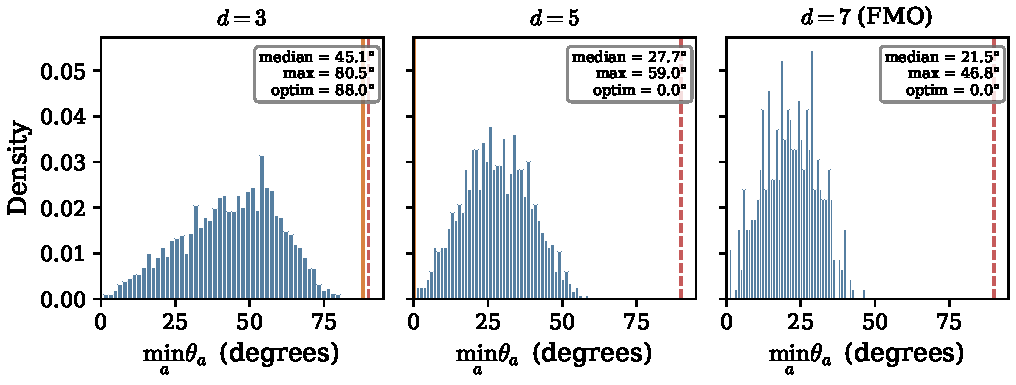
\includegraphics[width=\textwidth]{fig5_qudit_angles.pdf}
\caption{\textbf{Numerical illustration of Theorem~\ref{thm:global-orthogonality}.}  For each dimension $d \in \{3, 5, 7\}$, random full-rank density matrices are drawn from the Hilbert--Schmidt measure (blue histogram), and the minimum principal angle $\min_a \theta_a$ between the diagonal and off-diagonal tangent subspaces is computed via the Bures metric. The dashed red line marks $90^\circ$ (perfect orthogonality, achieved only at diagonal states). No non-diagonal state approaches orthogonality; the distribution shifts further from $90^\circ$ as $d$ increases. The orange line marks the best angle found by adversarial optimization. The $d = 7$ panel corresponds to the FMO Hilbert space dimension.}
\label{fig:qudit-angles}
\end{figure}

%% ============================================================
\section{Thermodynamic Cost of Decoherence}
\label{sec:thermodynamics}

\begin{proposition}[Free energy of coherence]
\label{prop:free-energy-coherence}
Let $\rho$ be a quantum state with system Hamiltonian $H$. The free energy change under dephasing is
\begin{equation}
\label{eq:free-energy-general}
F(\rho) - F(\Lambda_{\mathrm{dec}}[\rho]) = \mathrm{Tr}\bigl[(\rho - \Lambda_{\mathrm{dec}}[\rho]) H\bigr] + k_B T\, C_r(\rho),
\end{equation}
where $F(\rho) = \mathrm{Tr}[\rho H] - k_B T S(\rho)$ is the non-equilibrium free energy and $C_r(\rho) = S(\Lambda_{\mathrm{dec}}[\rho]) - S(\rho) \geq 0$ is the relative entropy of coherence \cite{streltsov2017colloquium}.
\end{proposition}

\begin{proof}
Direct rearrangement of $F(\rho) - F(\Lambda_{\mathrm{dec}}[\rho])$. Non-negativity of $C_r$ follows from unitality of $\Lambda_{\mathrm{dec}}$ and Schur-concavity of von Neumann entropy.
\end{proof}

When $H$ is diagonal in the dephasing basis, the energy term vanishes and
\begin{equation}
\label{eq:free-energy-diagonal-H}
F(\rho) - F(\Lambda_{\mathrm{dec}}[\rho]) = k_B T\, C_r(\rho) \geq 0.
\end{equation}
The free energy geometrically decomposes along the orthogonal subspaces of Theorem~\ref{thm:orthogonal-decomposition}: the classical component on $T_\rho^{\mathrm{diag}}$ and the coherent component on $T_\rho^{\mathrm{off}}$.

For a maximally coherent $d$-dimensional pure state, $C_r = \ln d$, and the cost per collapsed dimension is $k_B T \ln d/(d^2 - d) \approx k_B T \ln d / d^2$, which vanishes with system size---consistent with the extreme rapidity of macroscopic decoherence \cite{zurek2003decoherence}.

%% ============================================================
\section{Application to Photosynthetic Exciton Transport}
\label{sec:fmo}

\subsection{The FMO complex}
\label{sec:fmo-complex}

The Fenna--Matthews--Olson (FMO) complex of green sulfur bacteria (\textit{Chlorobaculum tepidum}) is a trimeric pigment-protein complex that channels excitation energy from the chlorosome antenna to the reaction center. Each monomer contains seven bacteriochlorophyll~\textit{a} (BChl~\textit{a}) chromophores whose excitonic couplings have been determined spectroscopically \cite{adolphs2006proteins}. The site-energy Hamiltonian in the site basis (energies in cm$^{-1}$ relative to $12\,210$\,cm$^{-1}$) is \cite{adolphs2006proteins}:
\begin{equation}
\label{eq:fmo-hamiltonian}
H_{\mathrm{FMO}} = \begin{pmatrix}
200 & -87.7 & 5.5 & -5.9 & 6.7 & -13.7 & -9.9 \\
-87.7 & 320 & 30.8 & 8.2 & 0.7 & 11.8 & 4.3 \\
5.5 & 30.8 & 0 & -53.5 & -2.2 & -9.6 & 6.0 \\
-5.9 & 8.2 & -53.5 & 110 & -70.7 & -17.0 & -63.3 \\
6.7 & 0.7 & -2.2 & -70.7 & 270 & 81.1 & -1.3 \\
-13.7 & 11.8 & -9.6 & -17.0 & 81.1 & 420 & 39.7 \\
-9.9 & 4.3 & 6.0 & -63.3 & -1.3 & 39.7 & 230
\end{pmatrix}.
\end{equation}
The dominant energy transfer pathways proceed as $1 \to 2 \to 3$ and $6 \to 5/7 \to 4 \to 3$, with site~3 serving as the exit site coupled to the reaction center \cite{adolphs2006proteins,cao2020quantum}. Decoherence due to protein-solvent fluctuations occurs on timescales of ${\sim}\,50$\,fs at physiological temperature \cite{cao2020quantum}, while excitation transfer completes in ${\sim}\,1$--$5$\,ps.

\subsection{Dimensional collapse in FMO}
\label{sec:fmo-collapse}

For the seven-site FMO complex ($d = 7$):
\begin{itemize}
\item Full quantum state space: $d^2 - 1 = 48$ real dimensions
\item Classical probability simplex: $d - 1 = 6$ dimensions
\item Collapse ratio: $1/(d+1) = 1/8 = 12.5\%$
\end{itemize}
Decoherence annihilates $d^2 - d = 42$ off-diagonal (coherence) dimensions---seven-eighths of the information-geometric degrees of freedom. The surviving 6-dimensional simplex encodes the classical site populations $\{p_1, \ldots, p_7\}$ (with $\sum_k p_k = 1$), which describe the probability of finding the excitation at each chromophore.

Under Haken--Strobl dephasing \cite{haken1973exactly} at rate $\gamma$ and trapping at the reaction-centre site~3 at rate $\Gamma_{\mathrm{trap}}$, the density matrix evolves as
\begin{equation}
\label{eq:lindblad}
\dot{\rho} = -\frac{i}{\hbar}[H_{\mathrm{FMO}}, \rho] + \gamma \sum_{k=1}^7 \left(|k\rangle\langle k| \rho |k\rangle\langle k| - \frac{1}{2}\{|k\rangle\langle k|, \rho\}\right) - \frac{\Gamma_{\mathrm{trap}}}{2}\{|3\rangle\langle 3|, \rho\}.
\end{equation}
The first term generates unitary evolution, the second dephases coherences at rate $\gamma$, and the third removes population into the reaction-centre sink ($\Gamma_{\mathrm{trap}} = 1\,\mathrm{ps}^{-1}$, following \cite{rebentrost2009environment}). The transport efficiency is $\eta = \Gamma_{\mathrm{trap}} \int_0^T \langle 3|\rho(t)|3\rangle\,dt$.

Since the trapping term makes the dynamics non-trace-preserving (population leaks irreversibly into the reaction centre), we define the \emph{conditional state} $\hat{\rho}(t) = \rho(t)/\mathrm{Tr}[\rho(t)]$---the state of the exciton conditioned on not yet having been trapped. This renormalized state is a proper density matrix to which the Bures metric and principal angle analysis apply. In the pure-dephasing limit ($H = 0$, $\Gamma_{\mathrm{trap}} = 0$), off-diagonal elements decay as $\rho_{kl} \to e^{-\gamma t}\rho_{kl}$; the full dynamics~\eqref{eq:lindblad} is a competition between coherent Hamiltonian evolution, incoherent dephasing, and trapping.

\subsection{Transport efficiency and ENAQT}
\label{sec:fmo-enaqt}

ENAQT \cite{rebentrost2009environment,plenio2008dephasing} occurs because pure quantum evolution can trap excitations in interference patterns, while moderate dephasing breaks destructive interference and opens transport channels. Figure~\ref{fig:fmo-collapse}(a) shows the transport efficiency $\eta(\gamma)$ computed from~\eqref{eq:lindblad} for both natural entry points: site~1 (from the baseplate) and site~6 (from the CsmA antenna).

Both initial conditions produce a clear ENAQT peak: efficiency rises from low values at $\gamma \to 0$ (quantum localization), reaches a maximum at $\gamma_{\mathrm{opt}} \approx 100$--$150$\,cm$^{-1}$, and slowly declines at large $\gamma$ (classical hopping limit). The optimal dephasing rate falls within the physiological range for FMO at 300\,K ($\gamma \sim 50$--$200$\,cm$^{-1}$ \cite{cao2020quantum}), consistent with the ENAQT literature \cite{rebentrost2009environment}.

\subsection{Geometry of the quantum-classical split}
\label{sec:fmo-geometry}

We now ask: what does the ENAQT regime look like in the information geometry of the quantum-classical transition?

For the FMO complex ($d = 7$), the diagonal and off-diagonal tangent subspaces have dimensions $d - 1 = 6$ and $d^2 - d = 42$ respectively, and their relative orientation is described by $d - 1 = 6$ principal angles $\theta_1 \leq \cdots \leq \theta_6$. We compute these at each dephasing rate $\gamma$ by evolving the full sink-inclusive model~\eqref{eq:lindblad} for 5\,ps, renormalizing the surviving state $\hat{\rho} = \rho/\mathrm{Tr}[\rho]$, and extracting the Bures-metric cross-Gram matrix between diagonal and off-diagonal basis directions (see Appendix). Figure~\ref{fig:fmo-collapse}(b) shows the minimum principal angle $\theta_{\min}(\gamma)$ for both site~1 and site~6 initial excitations.

The two initial conditions produce nearly identical angle curves, confirming that the geometric structure of the quantum-classical transition is robust to the choice of entry point. At weak dephasing ($\gamma \lesssim 1$\,cm$^{-1}$), the minimum principal angle drops below $50^\circ$: the classical population subspace and the quantum coherence subspace are far from orthogonal, meaning that population and coherence parameters are strongly mixed in the Fisher information sense. At moderate dephasing ($\gamma \sim 5$--$20$\,cm$^{-1}$), angles are in the range $70^\circ$--$85^\circ$. At the ENAQT optimal dephasing rate ($\gamma_{\mathrm{opt}} \approx 100$--$150$\,cm$^{-1}$), all six angles exceed $87^\circ$ and the state is geometrically close to classical. The dotted vertical lines in Figure~\ref{fig:fmo-collapse}(b) mark the efficiency-peak $\gamma$ values from panel~(a), showing that optimal transport occurs in a regime where the quantum-classical split is nearly orthogonal. Crucially, both panels are computed from the same sink-inclusive dynamics~\eqref{eq:lindblad}: the efficiency from accumulated trapped population, and the geometry from the renormalized conditional state $\hat{\rho}$.

This quantitative result reveals that ENAQT does not require a regime of strong quantum-classical mixing. The biologically relevant quantum effects arise from the \emph{small residual departure} from classical orthogonality: the system exploits the last few degrees of geometric non-orthogonality before full classical decoupling. The most geometrically interesting transition---where angles pass through $45^\circ$--$80^\circ$---occurs at dephasing rates ($\gamma \sim 1$--$20$\,cm$^{-1}$) well below the physiological range.

\begin{figure}[H]
\centering
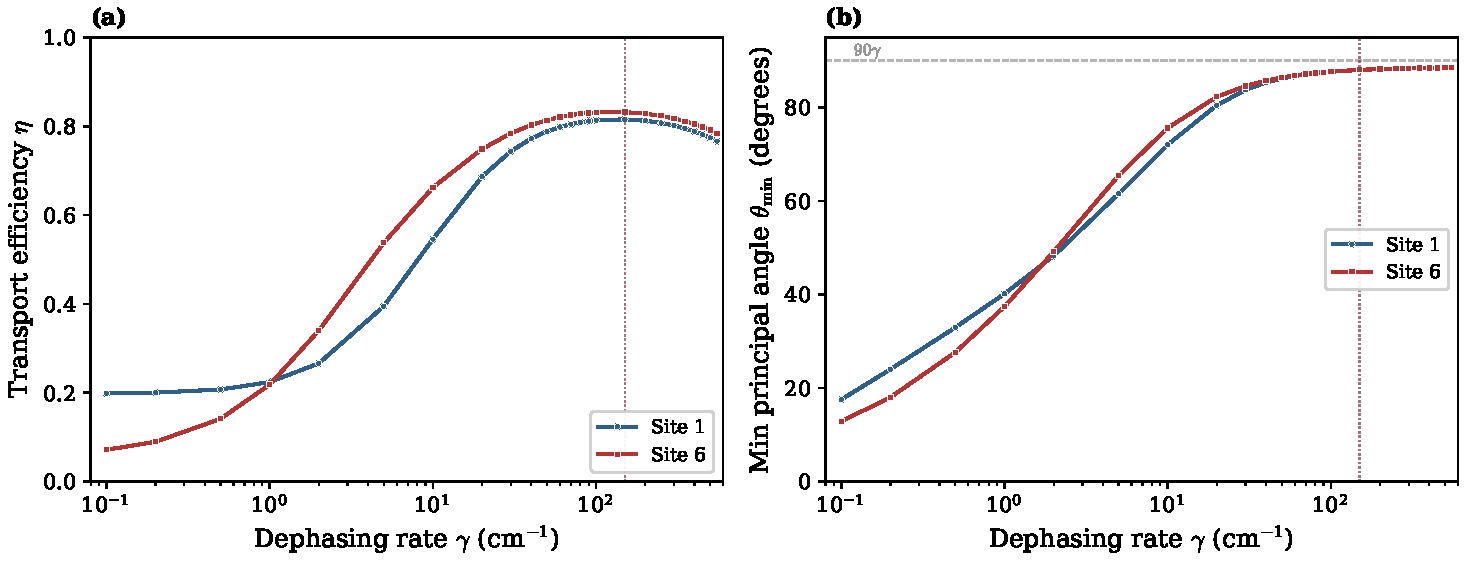
\includegraphics[width=\textwidth]{fig4_fmo_collapse.pdf}
\caption{\textbf{Transport efficiency and Bures geometry in the FMO complex.} Both panels use the same sink-inclusive dynamics~\eqref{eq:lindblad} with $\Gamma_{\mathrm{trap}} = 1$\,ps$^{-1}$. \textbf{(a)}~Transport efficiency $\eta$ as a function of Haken--Strobl dephasing rate $\gamma$. Both natural entry points (site~1, site~6) show a clear ENAQT peak at $\gamma_{\mathrm{opt}} \approx 100$--$150$\,cm$^{-1}$. \textbf{(b)}~Minimum Bures principal angle $\theta_{\min}$ between the diagonal and off-diagonal tangent subspaces, computed from the renormalized conditional state $\hat{\rho} = \rho/\mathrm{Tr}[\rho]$ at $t = 5$\,ps. Dotted vertical lines mark the efficiency-peak $\gamma$ from panel~(a). At the ENAQT optimum, all principal angles exceed $87^\circ$: optimal transport occurs in a regime that is geometrically close to classical.}
\label{fig:fmo-collapse}
\end{figure}

\subsection{FMO coupling graph}
\label{sec:fmo-graph}

The coupling structure of the FMO Hamiltonian can be represented as a graph where vertices are chromophore sites and edges connect pairs with significant electronic coupling ($|J_{kl}| > 5$\,cm$^{-1}$). Figure~\ref{fig:fmo-graph} shows this graph. Four site pairs have couplings below the 5\,cm$^{-1}$ threshold: (2,5), (2,7), (3,5), and (5,7), all involving sites at opposite ends of the two main transport pathways $1 \to 2 \to 3$ and $6 \to 5/7 \to 4 \to 3$.

\begin{figure}[H]
\centering
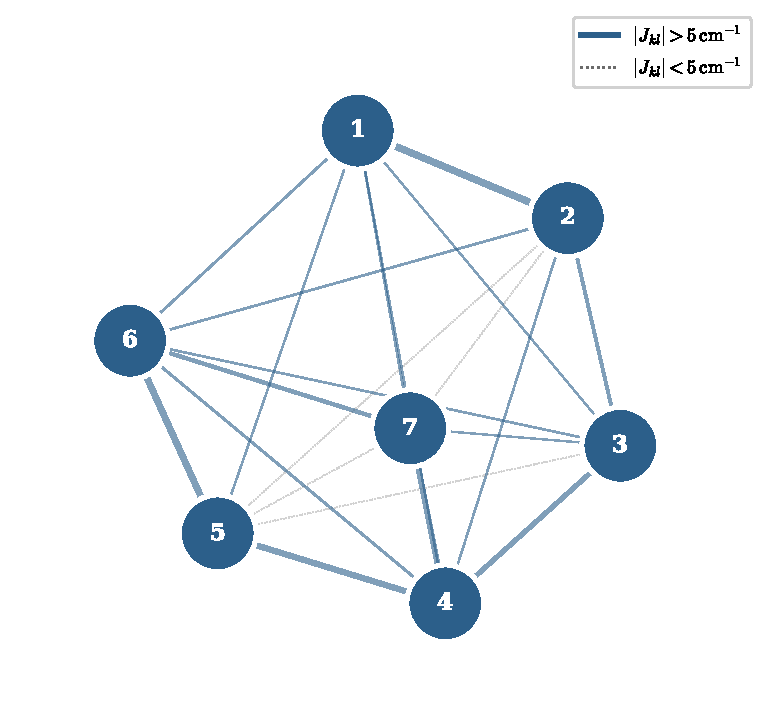
\includegraphics[width=0.6\textwidth]{fig2_fmo_graph.pdf}
\caption{\textbf{FMO coupling graph.} Vertices represent the seven BChl sites; edges connect pairs with significant coupling ($|J_{kl}| > 5$\,cm$^{-1}$). Edge widths are proportional to coupling strength. Dotted lines show weak couplings ($|J_{kl}| < 5$\,cm$^{-1}$). The four weak pairs all involve sites at opposite ends of the two main transport pathways.}
\label{fig:fmo-graph}
\end{figure}

%% ============================================================
\section{Discussion}
\label{sec:discussion}

\subsection{Summary of results}

We have shown that decoherence is a dimensional collapse in the information-geometric sense: $d^2 - 1 \to d - 1$ dimensions, with the Bures metric restricting to Fisher--Rao on the surviving simplex. The exact Bures separation angle quantifies the geometry of the classical-quantum split at every full-rank qubit state, and the global orthogonality theorem (Theorem~\ref{thm:global-orthogonality}) establishes that for $d \geq 3$ the diagonal and off-diagonal tangent subspaces are Bures-orthogonal at every non-diagonal state---resolving the higher-dimensional geometry exactly. Applied to the FMO complex with sink-inclusive dynamics, principal angle analysis reveals that at the ENAQT-optimal dephasing rate the system is geometrically close to classical (all principal angles $> 87^\circ$), while the strong quantum-classical mixing regime lies at much weaker dephasing ($\gamma \lesssim 10$\,cm$^{-1}$).

\subsection{Limitations}

The qubit separation angle (Theorem~\ref{thm:bures-angle}) is exact, and the global orthogonality theorem (Theorem~\ref{thm:global-orthogonality}) is sharp for all $d \geq 3$; the perturbative expansion (Theorem~\ref{thm:qudit-angles}) quantifies the departure from orthogonality but is limited to small coherence. The Haken--Strobl dephasing model used for FMO is simplified: the real protein-solvent bath has structured spectral density, non-Markovian dynamics, and spatially correlated fluctuations \cite{cao2020quantum}. The principal angles are computed on the renormalized conditional state $\hat{\rho} = \rho/\mathrm{Tr}[\rho]$; this is the natural object for the surviving exciton's geometry, but it means the Bures analysis inherits any artifacts of the Haken--Strobl model's treatment of system-bath correlations. Extending the information-geometric analysis to structured baths and non-Markovian dephasing is an open problem.

\subsection{Outlook}
\label{sec:bridge}

Theorem~\ref{thm:metric-restriction} establishes that the Fisher--Rao metric on the surviving classical simplex is the restriction of the Bures metric from the quantum state manifold. This geometric continuity suggests a natural question: whether classical coherence phenomena on longer timescales \cite{todd2026coherence,todd2026intelligence}---dissipative dynamics within the Fisher--Rao simplex---can be analyzed with the same information-geometric tools developed here. We leave this as a direction for future work.

\subsection{Open questions}

\begin{enumerate}
\item \emph{Non-Markovian geometry}: characterizing the dimensional collapse under structured (non-Markovian) dephasing, where coherence revivals temporarily restore collapsed dimensions.
\item \emph{Multi-chromophore entanglement}: extending beyond single-exciton states to multi-exciton manifolds, where inter-chromophore entanglement adds structure beyond site-basis coherence.
\item \emph{Quantum Darwinism}: the pointer states selected by einselection \cite{zurek2003decoherence,zurek2025decoherence} determine \emph{which} $(d{-}1)$-dimensional submanifold the collapse targets; the collapse magnitude is basis-independent.
\end{enumerate}

\bibliographystyle{unsrt}
\bibliography{references}

%% ============================================================
\appendix
\section{Numerical Methods}
\label{app:numerics}

\paragraph{Random state generation.}
Full-rank density matrices are drawn from the Hilbert--Schmidt measure: generate a $d \times d$ matrix $A$ with i.i.d.\ standard complex Gaussian entries, form $\rho = AA^\dagger/\mathrm{Tr}[AA^\dagger]$.

\paragraph{SLD computation.}
For each tangent direction $X$, the SLD $L_X$ satisfying $\rho L_X + L_X \rho = 2X$ is computed in the eigenbasis: $(L_X)_{mn}^{\mathrm{eig}} = 2X_{mn}^{\mathrm{eig}}/(\lambda_m + \lambda_n)$.

\paragraph{Principal angles.}
The $d - 1$ principal angles between $T_\rho^{\mathrm{diag}}$ and $T_\rho^{\mathrm{off}}$ are computed as $\theta_a = \arccos(\sigma_a)$, where $\sigma_1, \ldots, \sigma_{d-1}$ are the singular values of $G_{DD}^{-1/2} G_{DO} G_{OO}^{-1/2}$.

\paragraph{Adversarial search.}
$100$ L-BFGS-B optimizations per dimension maximize $\min_a \theta_a$ over full-rank parameterized states. No optimized state approaches $90^\circ$.

\paragraph{FMO dephasing simulation.}
The Lindblad master equation~\eqref{eq:lindblad} is integrated numerically using a fourth-order Runge--Kutta scheme with time step $\Delta t = 1.0$\,fs. The FMO Hamiltonian~\eqref{eq:fmo-hamiltonian} uses site energies and couplings from Adolphs and Renger \cite{adolphs2006proteins}. Both transport efficiency and principal angles are computed from the same sink-inclusive dynamics ($\Gamma_{\mathrm{trap}} = 1$\,ps$^{-1}$ at site~3). For the efficiency, accumulated trapped population is integrated over $t = 15$\,ps. For the principal angles, the density matrix is evolved for $t = 5$\,ps and the surviving state is renormalized: $\hat{\rho} = \rho/\mathrm{Tr}[\rho]$. Both initial conditions $\rho(0) = |1\rangle\langle 1|$ (site~1) and $\rho(0) = |6\rangle\langle 6|$ (site~6) are used to test robustness. For dephasing rates $\gamma \geq 5$\,cm$^{-1}$, the coherence decay time $\gamma^{-1} \lesssim 1$\,ps is shorter than the evolution time, ensuring coherences have reached a quasi-stationary balance. At physiological dephasing rates ($\gamma \geq 50$\,cm$^{-1}$), the minimum principal angle varies by less than $1.2^\circ$ across readout times of 3--8\,ps, confirming that the geometric conclusions are not sensitive to the choice of evolution window. The renormalized state is regularized to full rank ($\hat{\rho} \mapsto \hat{\rho} + 10^{-10}\,I/d$) before computing the six Bures principal angles between the diagonal and off-diagonal tangent subspaces.

\paragraph{Software.}
All computations use NumPy and SciPy. Source code is available in the repository.

\end{document}
